In der Matrixoptik werden Strahlen durch Vektoren mit zwei Elementen
dargestellt.
Ordnen Sie die Lichstrahlen in der Abbildung den folgenden Vektoren zu:

\def\punkt#1{
	\fill[color=white] #1 circle[radius=0.05];
	\draw[color=red] #1 circle[radius=0.05];
}
\def\aufgabenbild{
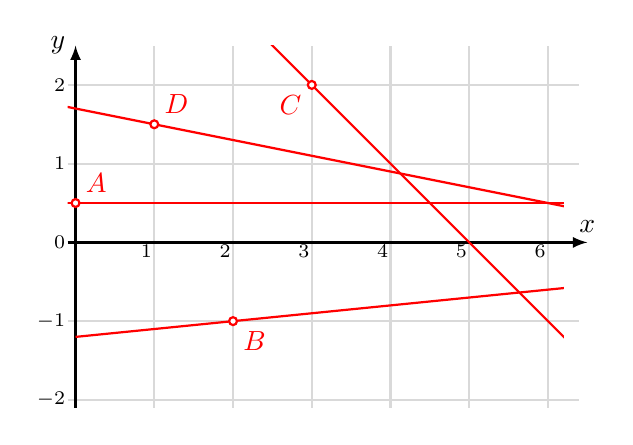
\begin{tikzpicture}[>=latex,thick]
\foreach \y in {-2,...,2}{
	\draw[color=gray!30] (-0.1,\y) -- (6.4,\y);
}
\foreach \x in {1,...,6}{
	\draw[color=gray!30] (\x,-2.1) -- (\x,2.5);
}
\draw[->] (-0.1,0) -- (6.5,0) coordinate[label={$x$}];
\draw[->] (0,-2.1) -- (0,2.5) coordinate[label={left:$y$}];
\begin{scope}
\clip (-0.1,-2.1) rectangle (6.2,2.5);
%
\draw[color=red] (-1,0.5) -- ++(8,0);
\punkt{(0,0.5)}
\node[color=red] at (0,0.5) [above right] {$A$};
%
\draw[color=red] (0,-1.2) -- (7,-0.5);
\punkt{(2,-1)}
\node[color=red] at (2,-1) [below right] {$B$};
%
\draw[color=red] (0,5) -- (7,-2);
\punkt{(3,2)}
\node[color=red] at (3,2) [below left] {$C$};
%
\draw[color=red] (-1,1.9) -- (7,0.3);
\punkt{(1,1.5)}
\node[color=red] at (1,1.5) [above right] {$D$};
\end{scope}

\node at (1.1,0.1) [below left] {$\scriptstyle 1$};
\node at (2.1,0.1) [below left] {$\scriptstyle 2$};
\node at (3.1,0.1) [below left] {$\scriptstyle 3$};
\node at (4.1,0.1) [below left] {$\scriptstyle 4$};
\node at (5.1,0.1) [below left] {$\scriptstyle 5$};
\node at (6.1,0.1) [below left] {$\scriptstyle 6$};
\node at (0,2) [left] {$\scriptstyle 2$};
\node at (0,1) [left] {$\scriptstyle 1$};
\node at (0,0) [left] {$\scriptstyle 0$};
\node at (0,-1) [left] {$\scriptstyle -1$};
\node at (0,-2) [left] {$\scriptstyle -2$};
\end{tikzpicture}}%

\begin{teilaufgaben}
\item
$\begin{pmatrix} \phantom{-}2 \\ -1 \end{pmatrix}$
\item
$\begin{pmatrix} \phantom{-}1.5 \\ -0.2 \end{pmatrix}$
\item
$\begin{pmatrix} -1\phantom{.0} \\ \phantom{-}0.1 \end{pmatrix}$
\item
$\begin{pmatrix} 0.5 \\ 0\phantom{.5} \end{pmatrix}$
\end{teilaufgaben}
\nopagebreak
\smash{\raisebox{0.0cm}{%
\hbox{\hspace*{4cm}%
\aufgabenbild
}}}

\begin{loesung}
\begin{teilaufgaben}
\item $C$
\item $D$
\item $B$
\item $A$
\qedhere
\end{teilaufgaben}
\end{loesung}
